\chapter{PCM Module Implementation}\label{chap:module}
This chapter will focus on the implementation of the PCM module within the GVSoC framework.
We will start by introducing the architecture of the module and the data-structures used to store the crossbar values.
Then we will analyse the MVM algorithm and how we can optimise it to achieve better performance.\\
The first step before starting the implementation is to define the constraints of the architecture and the software running the simulator.
\section{Architecture Constraints}\label{sec:arch_const}
Before analysing the module itself it's important to define some hardware constraints of the hardware running the simulator and software constraints of the simulator itself.
\subsection{Hardware Constraints}\label{sec:hw_const}
The hardware running the simulator spans across various architectures and configurations from low power laptops to HPC nodes and high power workstations.
This is a major concern when writing optimised code, especially when micro-optimisation are considered.
For this reason the optimisation will be maintained at a high level, avoiding architecture-specific optimisations and hardware accelerators usage.
\subsection{Software Constraints}\label{sec:sw_const}
The GVSoC framework is a C++ based SoC event simulator. While it supports many architectures and configurations, the software is intentionally single‑threaded to preserve event‑accurate simulations.
Clusters simulations on HPC nodes and high‑performance workstations reveal that the main bottlenecks are single‑thread performance and memory consumption. Therefore the optimisations will target both CPU efficiency and RAM usage.

\section{PCM Module Architecture}\label{sec:module_arch}
The PCM module architecture is shown figure \picref{fig:PCM-Module-Architecture} in the previous chapter.\\
To summarise, the module is characterised by a matrix of tiles. Each tile is a 3D array itself with surface $X \times Y$ and depth $K$, with $K$ being the 
number of layers of PCM cells stacked on top of each other. Each cell is able to holds $n$-bits as variable resistance.
The tiles are interfaced with a set of DACs connected to the rows and ADCs connected to the columns, enabling bidirectional conversion of input vectors from digital to analog and output vectors from analog to digital, respectively.
This is the basic architecture of the PCM module used in this implementation.
\section{Module Data-Structures}\label{sec:module_data}
Based on the architecture of our module we notice the need of a large memory bank capable of accommodating all the values.
To add an abstraction layer we can model only the layers and matrices sectors without major concern for the physical layer.
The primary issue is to define a data-structure to store all the weight stored in the matrice, to allow for a fully configurable design dynamically allocated arrays comes across as the first choice
However it's key to define a matrix-vector multiplication algorithm to immediately test whether the data-structure is effective.
\begin{equation}
Y_{s\cdot J + j}=\sum_{i=0}^{I-1}(\sum_{l\in L_s} M_{s,l,j,i}\cdot X_i)
\label{MVM_imp}
\end{equation}
Where:
\begin{conditions}
    s & sector index\\
    j & tile row index\\
    J & number of rows in the tile\\
    l & layer index\\
    i & column index\\
    L_s & layers used in the sector\\
    I & number of columns in the matrix\\
    M & matrix\\
    X & input vector\\
    Y & output vector
\end{conditions}
The above equation describe the MVM operation performed by the PCM module. It iterates over each enabled sector $s$ and for each row $j$ of the tile, 
it computes the dot product between the input vector $X$ and the corresponding row of the matrix $M$ across all enabled layers $L_s$.
We are going to use this naive implementation to make initial benchmarks to find the best data-structure.

\subsection{Data-structure Optimisation}\label{sec:data_opt}
The first step is to define a general data-structure that can be used to store the values of the PCM module.
\subsubsection{4D Array}\label{sec:4d_array}
An immediate solution would be to use a 4 dimension dynamically allocated array. 
Benefits from this architecture would be an easy access for each cells with a standard $n$-dimensional matrix approach.
However this structure is not optimal for major performance issues.
A multidimensional array dynamically allocated array can create cache locality issues that might revolve in more cache misses
than necessary slowing down the algorithm, moreover there is a high overhead in pointer allocations and deallocations during the lifetime of the model object.
Another major issue, even more crucial for this use case is not optimal memory usage, not only each allocation might not be contiguous in memory, leading to fragmentation and inefficient use of the available memory but also
pointer dereferencing and pointer arithmetic can lead to inefficient memory access patterns, especially for large dimensions of the matrix.

\subsubsection{Flat Buffer}\label{sec:flat_buf}
A second, more optimised, approach would be to use a "flat" $n$-dimensional array.
This solution require a more advanced indexing computation, however it resolve in far fewer instruction for both allocation and deallocation.
Implementing this solution show significant improvement in performance. Analysing a test program with valgrind cachegrind
 (a tool provided by the valgrind framework to simulate cache access) shows far fewer cache misses and and a fraction of memory reads.
The fewer cache misses are the result of the sequentially stored data followed by the memory sequentially read, reduced memory reads occur because contiguous memory allocation eliminates pointer dereference overhead.
One of the main drawback of this approach is the need to compute the index of each cell manually, however inline functions, macros and registers reuse strategies can help to reduce the complexity and the number of instructions required.

\subsection{Differential Algorithm}\label{sec:diff_algo}
Before moving to optimisations of the MVM algorithm it's important to note that the PCM module is capable of using differential weights.
This means that each weight is represented by two PCM cells, one for the positive part and one for the negative part the final weight is computed as the difference between the two cells.
This approach allows to maintain high precision despite the inevitable drift caused by the module physical characteristics.
To accommodate this feature, without changing the data-structure or the MVM algorithm, it's possible to use two computation passes.
\begin{equation}
Y_{s\cdot J + j}=\sum_{i=0}^{I-1}(M_{s,h_l,j,i}-M_{s,l_l,j,i})\cdot X_i = \sum_{i=0}^{I-1}M_{s,h_l,j,i}\cdot X_i -\sum_{i=0}^{I-1}M_{s,l_l,j,i}\cdot X_i
\end{equation}
Where:
\begin{conditions}
    h_l & High Layer\\
    l_l & Low Layer\\
\end{conditions}
This approach, while doubling the number of operations required, allows to maintain the same data-structure and MVM algorithm that we are going to optimise in the next section.
This trade-off is acceptable because the differential approach is not commonly used and the optimisations for one of the two cases are mutually beneficial.
\section{MVM Algorithm}\label{sec:mvm_algo}
In this section we are going to analyse and improve the MVM algorithm performances.
\subsection{Standard Implementation}\label{sec:std_imp}
The standard algorithm to compute a MVM using this PCM module, that is already described in the previous section [\ref{MVM_imp}]:
While some faster algorithms for sparse \cite{abboud_time_2023} and band matrix are describe in literature is notable that,
in this generalised case, the matrix does not adhere to any of those rules and keeping track of the non-zero elements would require additional memory, which is not optimal for our use case.
For this reason the optimisations will target the standard algorithm by working on the code and structures.\\

Looking at the data-structure we notice two main point. 
First of all the matrix is already divided in blocks (tiles) and sectors. 
As suggested by some studies \cite{yajnaseni_survey_2015} granularity is one of the key for fast MVMs and MMs algorithms. 
Secondly our MVMs compute row by vector, 
rows that are stored sequentialy in our flat buffer, meaning our data already follows cache friendly and granularity rules.
This implementation already offer performance speed-ups while closely simulating the PCM module.

\section{Optimisations}\label{sec:optim}
While this step is not necessary in a simulation environment it's key to run big simulations in a reasonable time even on low power devices enabling wider accessibility and usability.

\subsection{Improved Cache-friendliness}\label{sec:cache_friendly}
From the analysis of the standard implementation [\ref{MVM_imp}] there is still some room for improvement in the cache friendliness.
In particular the way layers and sectors are handled can be alligned to improve cache-friendliness.
\begin{equation}
    Y_{s\cdot J + j}=\sum_{l\in L_s}(\sum_{i=0}^{I-1} M_{s,l,j,i}\cdot X_i)
    \label{MVM_op}
\end{equation}
By moving the layer to the outer loop cache locality is improved, by computing each layer completely before moving to the next one we are able to access the data in a more sequential manner, leading to fewer cache misses and data reads.
This design change need to be accounted by the data-structure especially in the way layers and sectors are loaded into memory.
\begin{figure}
    \centering
    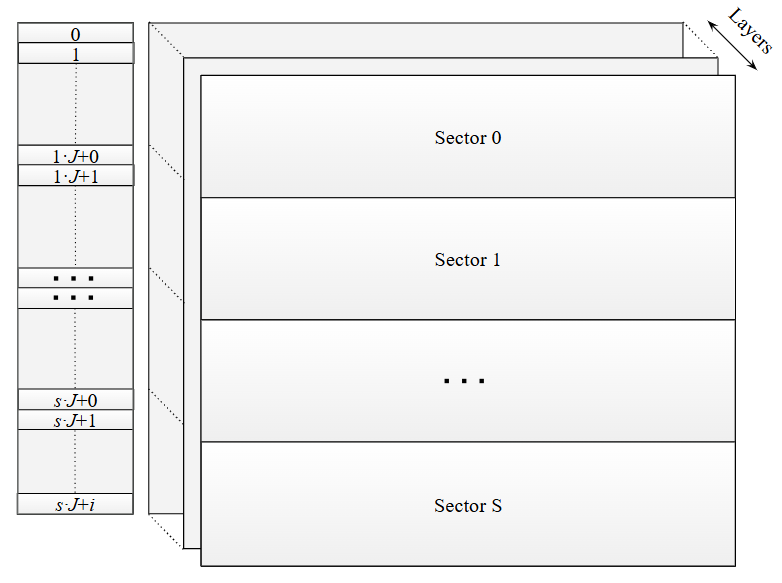
\includegraphics[width=0.5\textwidth]{Figures/pcm_cache_friendly.png}
    \caption{PCM matrix data-structure after cache-friendliness optimisation.}
    \label{fig:pcm_cache_friendly}
\end{figure}
\subsection{Register Reuse}\label{sec:reg_reuse}
Register reuse strategies are a great way to improve performance by reducing the number of memory accesses.
Specificly to this case, computing the sum of each row into a register without the need to store intermediate results in the output vector eliminates unnecessary memory writes and reads.
This approach lead to a significant reduction in memory accesses with the only drawback that is applicable only when the compiler is set to optimise the code.
Analysing the assembly code generated for each of the case it's immediate to see why.
In the non-optimised case the compiler store that same value on the stack and retrieves it at each iteration degrading the overall performances.\\

\lstdefinestyle{cleanasm}{
    language={[x86masm]Assembler},
    basicstyle=\tiny,
    keywordstyle=,
    commentstyle=,
    morekeywords={mov, push, lea, sub, add, cdqe},
    showstringspaces=false
}

\begin{table}[!ht]
\centering
\begin{minipage}[t]{.48\textwidth}
    \begin{lstlisting}[style=cleanasm,caption={Optimised Function Entry}]
        mov   r10, rdi
        push  r12
        lea   r9, [rcx+4]
        push  rbp
        mov   rbp, r8
        push  rbx
        mov   rbx, rdx
    \end{lstlisting}
\end{minipage}
\hfill
\begin{minipage}[t]{.48\textwidth}
    \begin{lstlisting}[style=cleanasm,caption={Un-Optimised Function Entry}]
        push  rbp
        mov   rbp, rsp
        push  rbx
        sub   rsp, 120
        mov   QWORD PTR [rbp-88], rdi
        mov   QWORD PTR [rbp-96], rsi
        mov   QWORD PTR [rbp-104], rdx
        mov   QWORD PTR [rbp-112], rcx
        mov   QWORD PTR [rbp-120], r8
    \end{lstlisting}
\end{minipage}

\vspace{0.5em} 

\begin{minipage}[t]{.48\textwidth}
    \begin{lstlisting}[style=cleanasm,caption={Optimised Variable Access}]
        movsx rdx, edi
        mov   r8, QWORD PTR [rbx+rdx*8]
    \end{lstlisting}
\end{minipage}
\hfill
\begin{minipage}[t]{.48\textwidth}
    \begin{lstlisting}[style=cleanasm,caption={Un-Optimised Variable Access}]
        mov   eax, DWORD PTR [rbp-24]
        cdqe
        lea   rdx, [0+rax*4]
        mov   rax, QWORD PTR [rbp-64]
        add   rax, rdx
        mov   eax, DWORD PTR [rax]
        mov   DWORD PTR [rbp-68], eax
    \end{lstlisting}
\end{minipage}

\caption{Comparison between optimised and un-optimised function setup and variable access code.}
\label{tab:asm_opt_comparison}
\end{table}
\subsection{Multithreading}\label{sec:multithread}
While cache-friendliness and register reuse are a great way to improve performance, multithreading is one of the best performance boosters in both MVMs and MMs.
\cite{yajnaseni_survey_2015,wyrzykowski_mathematical_2016,tang_multithreaded_2024,sulatycke_caching-efficient_1998}.
To both take advantage of multithreading, while minimising thread synchronisation and race conditions, that would slow down the algorithm, a modified implementation is proposed by moving some of the inner loops on different threads.
The loops in questions are the sector loops.
This approach guaranties granularity and, because each result value is stored at a different vector index,
there is no need to synchronise processes.
Moving to higher threads count than just the number of sectors is possible by splitting the row loop but require some synchronisation.
In this case atomic operations are used, the overhead is minimal because the atomic operation are limited to the write operation of the output vector however the performance impact is still present.

While implementing multithreading is fairly straight forward the problem lies in using the right amount of threads.
Some studies suggest that the number of threads should be equal to the number of physical cores \cite{bhutani_exploring_2024},
 using more threads will lead to "over-threading" and, therefore, worsen the performance.
However others studies suggests that the number of threads is, in small variation, independent of the number of physical cores and,
 especially in cases where synchronisation is not required, therefore suggesting that a different number of threads could be beneficial  \cite{cooper_how_2011}.
For this reason algorithm tests are proposed to investigate the optimal number of threads to use in the specific case
keeping in mind that the result aims to be as general as possible for consumer hardware.

\section{Digital to Analog \& Analog to Digital Converters}\label{sec:mod_gvsoc}
\subsection{DAC}\label{sec:dac}
The Digital to Analog Converter (DAC) is a key component of the PCM module, 
responsible for converting digital input vectors into analog signals that can be applied to the rows of the PCM array.
In this implementation, there is no need to simulate the actual analog signal because the PCM model, being simulated on a digital platform, can directly work with digital values.\\
It is important to note that the DAC introduces latency that is annotated as part of the simulation.
\subsection{ADC}\label{sec:adc}
The Analog to Digital Converter (ADC) is another key component of the PCM module,
responsible for converting the analog output signals from the columns of the PCM array back into digital values.
Similar to the DAC, in this implementation, there's no need to simulate the actual analog signal because the PCM model can directly work with digital values,
 however the ADC will clip the output values to the maximum and minimum values representable by the number of bits used in the conversion.
To model this behaviour, the ADC will apply a simple clipping function to the output values.
\begin{align}     
    n=output\;bit\;size\\
    ADC(y) = 
    \begin{cases}
    2^{n-1}-1 & \text{if } y > 2^{n-1}-1 \\
    -2^{n-1} & \text{if } y < -2^{n-1} \\
    y & \text{otherwise}
    \end{cases}
\end{align}
This function ensures that the output values are always within the valid range for the given output bit size.
Similar to the DAC, the ADC introduces latency that is annotated as part of the simulation.
\section{GVSoC Integration}\label{sec:gvsoc_int}
To integrate the PCM module into the GVSoC framework, we need to create a new peripheral class that represents the PCM.
This class will be responsible for handling the communication between the model and the rest of the system,
as well as managing the internal state of the PCM.
The PCM will be implemented as a memory-mapped peripheral, allowing the processor to read and write data to the PCM using standard memory access instructions.
The module will be connected to the system bus, allowing it to communicate with other peripherals and memory components in the system.
The bus interface will be implemented using the standard GVSoC wire.\\
The module have a defined mapping capable of exposing the memory space, read and write of the PCM cells, and the main AIMC unit, 
allowing the processor to store the input vector, trigger the MVM operation, write the input vector, and read the output vector.
All the operations will expose the result immediately by queuing the result at the correct time, the only exception is the MVM operation that while taking place immediately will expose the result after a defined latency once the event-timer that signals the module.
The PCM module will also include a set of configuration registers that allow the processor to configure the operation of the PCM module such as the MVM dimensions, weights precision and different MVM modes like signed and unsigned or the previously described differential mode.